\section{SNLI as a platform for NLI research}

The most immediate application for the SNLI corpus is in developing models for the task of NLI. In particular, since SNLI is dramatically larger than any existing corpus of comparable quality, we expect it to make possible the use of parameter-rich models like neural networks for this task. In this section, we explore the performance of a range of standard and novel models trained on the corpus.

\subsection{Standard entailment models}
We evaluate a number of strong baselines on the SNLI corpus.
The first class of baselines use models from the Excitement Open
  Platform (EOP,
  \citealt{pado2014design,magnini2014excitement})
  -- an open source platform for RTE research which
  is distributed alongside a number of RTE pipelines.
We additionally evaluate against a both an unlexicalized and lexicalized
  classifier with straightforward feature sets.
\todo{some meaningful insight from \#s}


%
% EOP
%
\paragraph{Excitement Open Platform}
% what is EOP
The Excitement Open Platform is a tool to quickly develop RTE systems
  while sharing components such as common lexical resources and 
  evaluation sets.
% 9 systems compared against
A number of systems have been built using the platform, 9 of them
  applicable to English are publicly distributed with version 1.2.1
  of the software.
% these fall into 2 classes
These fall into two classes of algorithms: 2 are edit distance based,
  whereas the remaining 7 make use of different features in a
  maximum entropy classifier.

% methodology
We convert the 3-way classification task in SNLI into the RTE setting
  by labeling both the \unknown\ and \contradiction\
  labels as negative entailment, and treating the \entailment\ label as
  the positive entailment.
This creates a biased dataset of 66\% negative examples.
% we report the best results from each class
We run each of the 9 algorithms distributed with EOP on the 2-class
  SNLI dataset, and report results for the best edit distance 
  configuration and the best classifier based configuration, as
  determined by performance on the development set.
\todo{we may not have CPU time for this}.

%
% EOP RESULTS TABLE
%
% Some definitions
\def\t#1{\small{#1}}
\def\b#1{\t{\textbf{#1}}}
\def\colspaceS{2.0mm}
\def\colspaceM{3.0mm}
\def\colspaceL{4.0mm}

% The table
\begin{table}
\begin{center}
\begin{tabular}{l@{\hskip \colspaceL}c@{\hskip \colspaceS}c@{\hskip \colspaceS}c@{\hskip \colspaceS}c@{\hskip \colspaceL}c@{\hskip \colspaceS}c}
\hline
\textbf{System} & \multicolumn{4}{c}{\b{SNLI}} & \multicolumn{2}{c}{\b{RTE-3}} \\
 & \t{P} & \t{R} & \t{F$_1$} & \t{Acc.} & \t{F$_1$} & \t{Acc.} \\
\hline
\t{Edit Distance} & \t{??.?} & \t{??.?} & \t{??.?} & \t{??.?} & 
                    \t{??.?} & \t{??.?} \\
\t{Classifier}    & \t{68.0} & \t{38.7} & \t{49.3} & \t{73.5} & 
                    \t{64.2} & \t{65.3} \\
\hline
\end{tabular}
\end{center}
% The caption
\caption{
\label{tab:eopresults}
2-class accuracy and precision/recall of existing competitive RTE
systems from the Excitement Open Platform.
Results are reported for an edit-distance based algorithm, and a
  classifier-based system.
For comparision, results are also reported on the RTE-3 dataset.
\todo{numbers are approx.}
}
\end{table}
%
% END EOP RESULTS TABLE
%

% the best systems
We report results in \reftab{eopresults}.
The best edit distance algorithm tunes the the weight of the three 
  case-insensitive edit distance operations on the training set, 
  after removing stop words.
The best classifier-based system \todo{does something}.
\todo{some insight from results}.

%
% Lexicalized Classifier
%
\paragraph{Lexicalized Classifier}
Unlike the RTE datasets, SNLI's size allows approaches which make use of
  rich lexicalized features.
We implmement a lexicalized classifier to provide a strong baseline for future work
  on the dataset.
Our classifier implements 6 features:
\begin{enumerate}  % TODO(gabor) This takes up way too much space
\setlength\itemsep{0em}
  \item the BLEU score of the \hypothesis\ with respect
  to the \premise, using an n-gram length between 1 and 4.

  \item The length difference between the \hypothesis\ and the \premise, as a real-valued
  feature.

  \item The overlap between words in the \premise\ and \hypothesis. This is counted
  both as an absolute count and a percentage of possible overlap, and is computed
  both over all words and over just nouns, verbs, adjectives, and adverbs.

  \item For every pair of words across the \premise\ and \hypothesis\ which share a 
  POS tag, an indicator feature over the two words.
  
  \item For every pair of bigrams across the \premise\ and \hypothesis\ which share a 
  POS tag, an indicator feature over the two bigrams.
  
  \item An indicator for every unigram and bigram in the \hypothesis.
\end{enumerate}

%
% BOW RESULTS TABLE
%
% Some definitions
\def\t#1{\small{#1}}
\def\b#1{\t{\textbf{#1}}}
\def\colspaceS{2.0mm}
\def\colspaceM{3.0mm}
\def\colspaceL{4.0mm}

% The table
\begin{table}
\begin{center}
\begin{tabular}{l@{\hskip \colspaceL}c@{\hskip \colspaceS}c@{\hskip \colspaceS}c@{\hskip \colspaceS}c@{\hskip \colspaceL}c}
\hline
\textbf{System} & \multicolumn{4}{c}{\b{2-Class}} & \b{3-Class} \\
 & \t{P} & \t{R} & \t{F$_1$} & \t{Acc.} & \t{Acc.} \\
\hline
\t{Lexicalized}            & \t{??.?} & \t{??.?} & \t{??.?} & \t{??.?} & \t{77.3} \\
\t{Unigrams Only}          & \t{??.?} & \t{??.?} & \t{??.?} & \t{??.?} & \t{??.?} \\
\t{Unlexicalized}          & \t{??.?} & \t{??.?} & \t{??.?} & \t{??.?} & \t{??.?} \\
\hline
\end{tabular}
\end{center}
% The caption
\caption{
\label{tab:bowresults}
Accuracy on the 2-class and 3-class SNLI dataset, as well as precision/recall
  on the 2-class task to allow for comparision with the RTE systems.
Ablation studies are reported for removing bigram features and all lexical
  features.
\todo{numbers are approx.}
}
\end{table}
%
% END BOW RESULTS TABLE
%

% Commenting out until PDF available. -S
%\Fig{learning_curves_bow.pdf}{0.6}{bowlearncurve}{
%A learning curve for the lexicalized and unlexicalized baseline classifiers.
%Note the y axis starting at a random-chance accuracy of 33\%.
%\todo{numbers are approx.}
%}

% Results
We report results in \reftab{bowresults}, along with ablation studies for removing
  the bigram features (leaving only the unigram entailment pair feature),
  and for removing all lexicalized features.
In addition, we report learning curves for the lexicalized and fully unlexicalized
  classifiers in \reffig{bowlearncurve}.

Note that \todo{something interesting happens}.


%\subsection{Existing NLI systems}

\subsection{Sentence embeddings and NLI}\label{sentence-embedding}

SNLI is uniquely suitable for training neural network models that produce vector representations of sentence meaning. In this section, we compare the performance of six such models on SNLI. 
In order to best evaluate the strengths of these six models at producing informative representations, we use sentence embedding as an intermediate step in the NLI classification task: each model most produce vector representation of each of the two sentences without using any context from the other sentence, and the two resulting vectors are then passed to a neural network classifier which predicts the label for the pair. This choice allows us to focus on evaluating the ability of existing models to produce representations that fully capture sentence meaning, at the possible cost of excluding from consideration neural models for NLI that directly compare the two inputs at the word or phrase level.


\begin{figure}[tp]
  \centering
\scalebox{0.85}{
 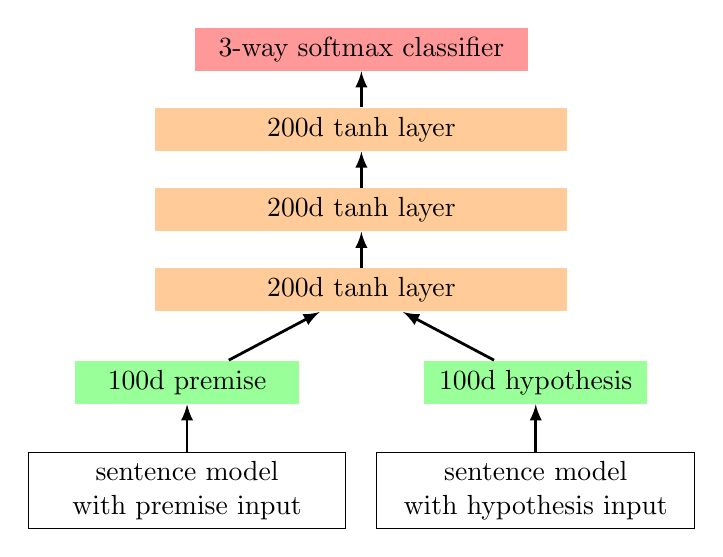
\begin{tikzpicture}
    \def\dx{21pt}
    \def\dy{29pt}

    \tikzstyle{label}=[text width=40mm,align=center]    
    \tikzstyle{softmax}=[fill=red!40,text width=40mm,align=center]
    \tikzstyle{preclass}=[fill=orange!40,text width=50mm,align=center]
    \tikzstyle{e}=[fill=green!40,text width=26mm,align=center]
    \tikzstyle{m}=[draw=black,text width=38mm,align=center]    
    
    \node[softmax]  (softmax) at (0*\dx,6*\dy) {3-way softmax classifier};
    \node[preclass]  (pc3) at (0*\dx,5*\dy) {200d $\tanh$ layer};
    \node[preclass]  (pc2) at (0*\dx,4*\dy) {200d $\tanh$ layer};
    \node[preclass]  (pc1) at (0*\dx,3*\dy) {200d $\tanh$ layer};
    \node[e]  (pe) at (-3*\dx,1.85*\dy) {100d premise};
    \node[e]  (he) at (3*\dx,1.85*\dy) {100d hypothesis};
    \node[m]  (pem) at (-3*\dx,0.5*\dy) {sentence model\\ with premise input};
    \node[m]  (hem) at (3*\dx,0.5*\dy) {sentence model\\ with hypothesis input};    
    
    \pgfsetarrowsend{latex}
    \tikzstyle{fwd} = [draw=black, line width=1pt]

          \draw [fwd] (pc3) -- (softmax);
          \draw [fwd] (pc2) -- (pc3);
          \draw [fwd] (pc1) -- (pc2);
          \draw [fwd] (pe) -- (pc1);
          \draw [fwd] (he) -- (pc1);
          \draw [fwd] (hem) -- (he);
          \draw [fwd] (pem) -- (pe);

  \end{tikzpicture}}
	
        \caption{The neural network classification architecture: for each sentence embedding model evaluated in \reftabs{tab:nnresults}{tab:transferresults}, two identical copies of the model are run with the two sentences as input, and their outputs are used as the two 100d inputs shown here.}
  \label{modelstructure}
\end{figure}

Our neural network classifier, depicted in Fig.~\ref{modelstructure} is simply a stack of three 100d $\tanh$ layers, with the bottom layer taking the concatenated sentence representations as input and the top layer feeding a softmax classifier, all trained jointly with the representation model itself.

We test six sentence representation models, each set to use 50d word and phrase embeddings. Our baseline model in this experiment simply sums the embeddings of the word in each sentence. Next, we experiment with two recurrent models: a plain RNN, and a one-layer LSTM RNN \cite{hochreiter1997long}. Finally, we experiment with three tree-structured models: a plain TreeRNN \cite{socher2011semi}, a tensor-parameterized TreeRNTN \cite{socher2013acl1}, and a TreeLSTM \cite{tai2015improved}.

The word embeddings for all of the moedels are initialized the 200d reference GloVe vectors \cite{pennington2014glove} and fine tuned. In addition, all of the models use an additional $\tanh$ neural network layer to map these 200d embeddings into the 50d working space. All of the models are randomly initialized using standard techniques and trained using AdaDelta \cite{zeiler2012adadelta} minibatch SGD until performance on the development set stops improving. We applied L2 regularization to all models, manually tuning the strength coefficient $\lambda$ for each. All models were reimplemented in a common framework for this paper, and the implementations will be made available at publication time.

\begin{table}
\begin{center}
\begin{tabular}{l@{\hskip \colspaceL}@{\hskip \colspaceL}c@{\hskip \colspaceL}c}
\hline
\textbf{Sentence model} & \b{Train}  & \b{Test}\\
\hline
\t{Sum of words}            & \t{} & \t{} \\
\t{RNN}            & \t{} & \t{} \\
\t{LSTM RNN}            & \t{75?} & \t{72?} \\
\t{TreeRNN}            & \t{} & \t{} \\
\t{TreeRNTN}            & \t{58?} & \t{56?} \\
\t{LSTM TreeRNN}            & \t{72?} & \t{69?} \\
\hline
\end{tabular}
\end{center}
% The caption
\caption{
\label{tab:nnresults}
Accuracy in 3-class classification on the SNLI training and test sets for each model.
\todo{Replace with final numbers}
}
\end{table}

Note that \todo{something interesting happens}.
